% Standalone preview and copy source for improved AdLint paper figures.
%
% Integration note:
% - Copy the "Shared figure styles" block into docs/adlint_hybrid_eval_paper.tex
%   after the existing color and \metricnote definitions.
% - Replace the existing figure environments with the matching blocks below.
% - The figures use current data from docs/adlint_hybrid_eval_paper.tex and avoid
%   \resizebox so labels are set at their final paper size.

\documentclass[11pt]{article}

\usepackage[
  letterpaper,
  top=0.85in,
  bottom=1.05in,
  left=1.18in,
  right=1.18in
]{geometry}
\usepackage[T1]{fontenc}
\usepackage{newpxtext}
\usepackage{newpxmath}
\usepackage[scale=0.94]{tgheros}
\usepackage{microtype}
\usepackage{graphicx}
\usepackage[table]{xcolor}
\usepackage{tikz}
\usepackage{pgfplots}
\usepackage[font={small,sf},labelfont={bf},labelsep=period]{caption}

\pgfplotsset{compat=1.18}
\usetikzlibrary{arrows.meta, backgrounds, calc, positioning}

\definecolor{adlintink}{HTML}{111827}
\definecolor{adlintmuted}{HTML}{4B5563}
\definecolor{adlintline}{HTML}{D1D5DB}
\definecolor{adlintsoft}{HTML}{F6F8FA}
\definecolor{adlintnavy}{HTML}{0F172A}
\definecolor{oiBlue}{HTML}{0072B2}
\definecolor{oiSky}{HTML}{56B4E9}
\definecolor{oiGreen}{HTML}{009E73}
\definecolor{oiOrange}{HTML}{E69F00}
\definecolor{oiVermillion}{HTML}{D55E00}
\definecolor{oiPurple}{HTML}{CC79A7}

\AtBeginDocument{\color{adlintink}}
\captionsetup{skip=0.45em}
\newcommand{\metricnote}[1]{\textcolor{adlintmuted}{\sffamily\footnotesize #1}}

% Shared figure styles --------------------------------------------------------
\colorlet{AdLintRule}{oiBlue}
\colorlet{AdLintModel}{oiOrange}
\colorlet{AdLintReport}{oiGreen}
\colorlet{AdLintEval}{oiPurple}
\colorlet{AdLintRisk}{oiVermillion}

\newcommand{\AdLintFigureFont}{\sffamily\small}
\newcommand{\AdLintTickFont}{\sffamily\footnotesize}
\newcommand{\AdLintValueLabel}[1]{%
  \pgfmathprintnumber[fixed,precision=#1,zerofill]{\pgfplotspointmeta}%
}

\tikzset{
  adlint flow box/.style={
    rounded corners=2pt,
    line width=0.65pt,
    align=center,
    inner xsep=5pt,
    inner ysep=5pt,
    minimum width=2.95cm,
    minimum height=1.08cm,
    text width=2.68cm,
    font=\AdLintFigureFont
  },
  adlint rule box/.style={adlint flow box, draw=AdLintRule, fill=AdLintRule!7},
  adlint model box/.style={adlint flow box, draw=AdLintModel, fill=AdLintModel!9},
  adlint report box/.style={adlint flow box, draw=AdLintReport, fill=AdLintReport!8},
  adlint eval box/.style={adlint flow box, draw=AdLintEval, fill=AdLintEval!8},
  adlint arrow/.style={
    -{Latex[length=2.1mm,width=1.55mm]},
    line width=0.65pt,
    draw=adlintmuted,
    rounded corners=2pt
  },
  adlint lane label/.style={
    font=\sffamily\scriptsize\bfseries,
    text=adlintmuted,
    anchor=west
  }
}

\pgfplotsset{
  adlint proposal axis/.style={
    font=\AdLintFigureFont,
    axis line style={adlintline},
    tick style={adlintline},
    tick label style={font=\AdLintTickFont, text=adlintmuted},
    label style={font=\AdLintFigureFont, text=adlintmuted},
    title style={font=\sffamily\small\bfseries, text=adlintnavy},
    grid style={adlintline!55},
    major grid style={adlintline!55},
    axis x line*=bottom,
    axis y line*=left,
    clip=false,
    every axis plot/.append style={line width=0.75pt}
  },
  adlint horizontal bars/.style={
    adlint proposal axis,
    xbar,
    width=0.80\linewidth,
    bar width=11pt,
    enlarge y limits=0.30,
    xmajorgrids=true,
    ymajorgrids=false,
    nodes near coords,
    point meta=x,
    nodes near coords style={
      font=\AdLintTickFont\bfseries,
      text=adlintnavy,
      anchor=west,
      xshift=2pt
    }
  }
}

\begin{document}

\section*{\sffamily AdLint Paper Figure Replacement Proposals}

\noindent{\sffamily\small
These figure environments preserve the current paper data while improving label
size, spacing, and color contrast. The palette stays within the existing
Okabe--Ito colors already defined by the paper.
}

% Replacement for Figure: Hybrid review architecture -------------------------
\begin{figure}[ht]
\centering
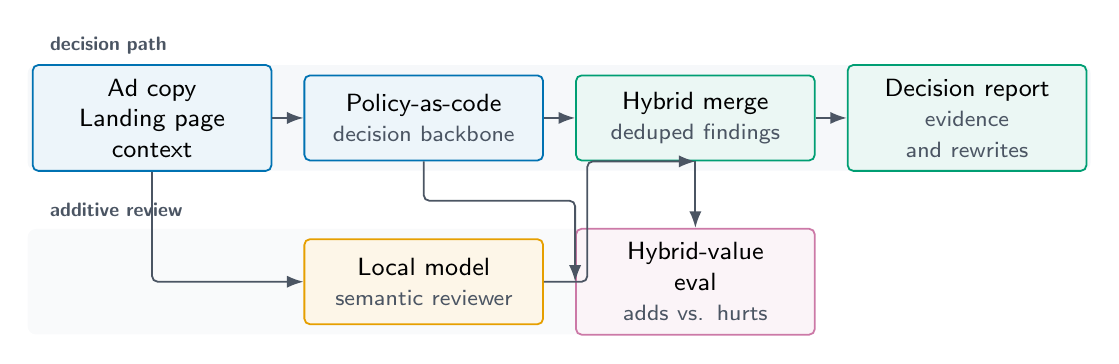
\begin{tikzpicture}[x=1cm,y=1cm]
\node[adlint lane label] at (-1.42,0.92) {decision path};
\node[adlint lane label] at (-1.42,-1.16) {additive review};

\node[adlint rule box] (input) at (0,0)
  {Ad copy\\Landing page\\context};
\node[adlint rule box] (rules) at (3.45,0)
  {Policy-as-code\\\metricnote{decision backbone}};
\node[adlint report box] (merge) at (6.90,0)
  {Hybrid merge\\\metricnote{deduped findings}};
\node[adlint report box] (report) at (10.35,0)
  {Decision report\\\metricnote{evidence and rewrites}};

\node[adlint model box] (model) at (3.45,-2.08)
  {Local model\\\metricnote{semantic reviewer}};
\node[adlint eval box] (eval) at (6.90,-2.08)
  {Hybrid-value\\eval\\\metricnote{adds vs. hurts}};

\draw[adlint arrow] (input) -- (rules);
\draw[adlint arrow] (rules) -- (merge);
\draw[adlint arrow] (merge) -- (report);
\draw[adlint arrow] (input.south) |- ($(model.west)+(-0.12,0)$) -- (model.west);
\draw[adlint arrow] (model.east) -- ++(0.55,0) |- (merge.south);
\draw[adlint arrow] (rules.south) -- ++(0,-0.50) -| (eval.west);
\draw[adlint arrow] (merge.south) -- (eval.north);

\begin{scope}[on background layer]
  \fill[adlintsoft, rounded corners=3pt]
    (-1.58,-0.67) rectangle (11.92,0.67);
  \fill[adlintsoft!70, rounded corners=3pt]
    (-1.58,-2.75) rectangle (8.42,-1.41);
\end{scope}
\end{tikzpicture}
\caption{Hybrid review architecture. Rules stay on the decision path; the local
model adds review signal and is evaluated for incremental value.}
\label{fig:architecture}
\end{figure}

% Replacement for Figure: Decision-label distribution ------------------------
\begin{figure}[ht]
\centering
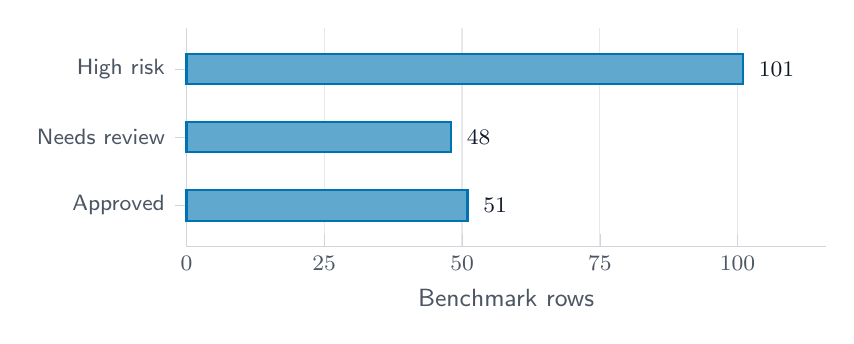
\begin{tikzpicture}
\begin{axis}[
  adlint horizontal bars,
  height=4.35cm,
  xmin=0,
  xmax=116,
  xlabel={Benchmark rows},
  symbolic y coords={Approved,Needs review,High risk},
  ytick=data,
  yticklabel style={font=\AdLintTickFont, text=adlintmuted, align=right},
  xtick={0,25,50,75,100},
  nodes near coords={\AdLintValueLabel{0}},
]
\addplot[fill=AdLintRule!62, draw=AdLintRule] coordinates {
  (51,Approved)
  (48,Needs review)
  (101,High risk)
};
\end{axis}
\end{tikzpicture}
\caption{Decision-label distribution in the 209-example rule benchmark.}
\label{fig:decision-distribution}
\end{figure}

% Replacement for Figure: Category-level precision ---------------------------
\begin{figure}[ht]
\centering
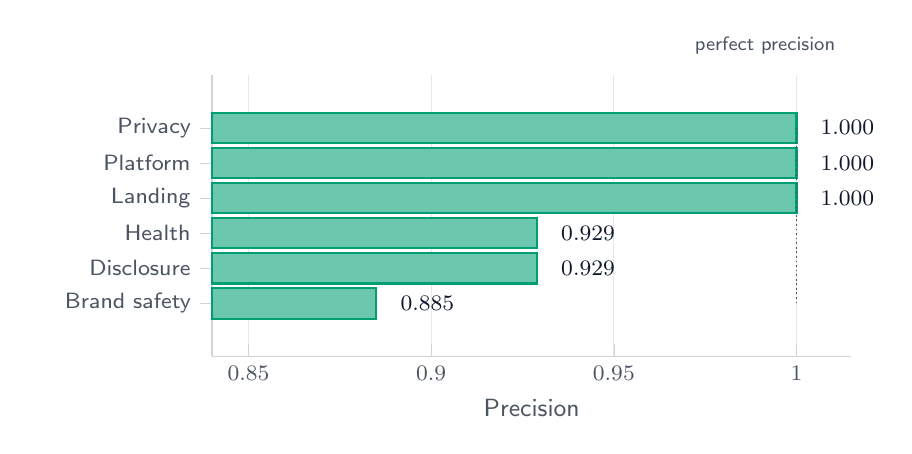
\begin{tikzpicture}
\begin{axis}[
  adlint horizontal bars,
  height=5.15cm,
  xmin=0.84,
  xmax=1.015,
  xlabel={Precision},
  symbolic y coords={Brand safety,Disclosure,Health,Landing,Platform,Privacy},
  ytick=data,
  yticklabel style={
    font=\AdLintTickFont,
    text=adlintmuted,
    align=right,
    text width=1.95cm
  },
  xtick={0.85,0.90,0.95,1.00},
  xticklabel style={/pgf/number format/fixed,/pgf/number format/precision=2},
  nodes near coords={\AdLintValueLabel{3}},
  every node near coord/.append style={xshift=3pt},
]
\addplot[fill=AdLintReport!58, draw=AdLintReport] coordinates {
  (0.885,Brand safety)
  (0.929,Disclosure)
  (0.929,Health)
  (1.000,Landing)
  (1.000,Platform)
  (1.000,Privacy)
};
\draw[densely dotted, draw=adlintmuted, line width=0.65pt]
  (axis cs:1.000,Brand safety) -- (axis cs:1.000,Privacy);
\node[anchor=south east, font=\sffamily\scriptsize, text=adlintmuted]
  at (axis description cs:0.99,1.04) {perfect precision};
\end{axis}
\end{tikzpicture}
\caption{Category-level precision for selected benchmark categories. Recall was
1.000 for all categories shown.}
\label{fig:category-precision}
\end{figure}

% Replacement for Figure: Smoke-run accuracy ---------------------------------
\begin{figure}[ht]
\centering
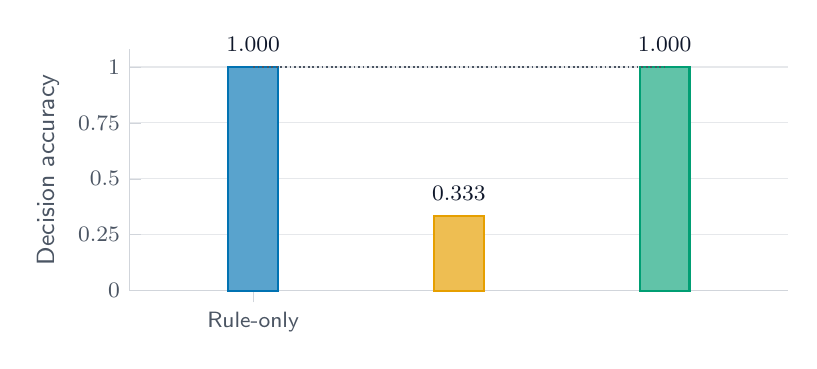
\begin{tikzpicture}
\begin{axis}[
  adlint proposal axis,
  ybar,
  width=0.82\linewidth,
  height=4.65cm,
  ylabel={Decision accuracy},
  ymin=0,
  ymax=1.08,
  symbolic x coords={Rule-only,Model-only,Hybrid},
  xtick=data,
  xticklabel style={font=\AdLintTickFont, text=adlintmuted, align=center},
  ytick={0,0.25,0.50,0.75,1.00},
  yticklabel style={/pgf/number format/fixed,/pgf/number format/precision=2},
  ymajorgrids=true,
  xmajorgrids=false,
  bar width=18pt,
  enlarge x limits=0.30,
  nodes near coords={\AdLintValueLabel{3}},
  point meta=y,
  nodes near coords style={
    font=\AdLintTickFont\bfseries,
    text=adlintnavy,
    anchor=south,
    yshift=2pt
  }
]
\addplot[ybar, bar shift=0pt, fill=AdLintRule!65, draw=AdLintRule]
  coordinates {(Rule-only,1.000)};
\addplot[ybar, bar shift=0pt, fill=AdLintModel!68, draw=AdLintModel]
  coordinates {(Model-only,0.333)};
\addplot[ybar, bar shift=0pt, fill=AdLintReport!62, draw=AdLintReport]
  coordinates {(Hybrid,1.000)};
\draw[densely dotted, draw=adlintmuted, line width=0.65pt]
  (axis cs:Rule-only,1.000) -- (axis cs:Hybrid,1.000);
\end{axis}
\end{tikzpicture}
\caption{Decision accuracy by mode in the local-model smoke run.}
\label{fig:smoke-accuracy}
\end{figure}

\end{document}
